\documentclass{article}
\usepackage{tikz}
\usepackage{listings}
\usepackage[utf8]{inputenc}
\usepackage{ amssymb }
\usepackage{amsfonts}
\usepackage{graphicx}
\usepackage{boxproof}
\usetikzlibrary{automata,positioning,arrows}

\title{Lógica Matemática. \\Tarea 3}
\author{Fabián Romero Jiménez}
\date{}
\begin{document}
\lstset{basicstyle=\footnotesize}
\maketitle
\begin{enumerate}

\item[\bf{Problema 1}] Considera el siguiente modelo de Kripke $(\mathcal{S,R,L})$ donde:
\begin{enumerate}
\item El conjunto de estados $\mathcal{S}$ es: $\{s_0, s_1, s_2, s_3\}$,
\item La relación de accesibilidad $\mathcal{R}$ es: $\{(s_0, s_0), (s_0, s_1), (s_0, s_3), (s_1, s_2), (s_2, s_1), (s_3, s_2)\}$
\item La función de etiquetamento $\mathcal{L}$ está dada por: $\mathcal{L}(s0) = \{r\}, \mathcal{L}(s1) = \{p,r\}, \mathcal{L}(s2) = \{q,r\}, \mathcal{L}(s_3) = \{p, q\}.$
\end{enumerate}

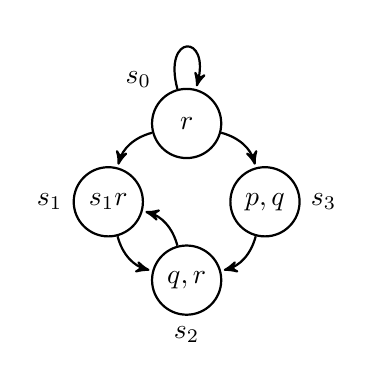
\begin{tikzpicture}[->,>=stealth',shorten >=1pt,auto,node distance=0.5cm,
  thick,main node/.style={circle,fill=blue!20,draw,font=\sffamily\Large\bfseries}]
   \node[state] (s_1) [label=left:$s_1$]  {$s_1 r$}; 
   \node[state] (s_0) [above right=of s_1,label=above left:$s_0$] {$r$};
   \node[state] (s_2) [below right=of s_1,label=below:$s_2$] {$q,r$};
   \node[state] (s_3) [above right=of s_2,label=right:$s_3$] {$p,q$};
    \path[->] 
    (s_1) edge  [bend right] node {} (s_2)
    (s_0) edge  [bend right] node {} (s_1)
          edge  [bend left] node {} (s_3)
          edge [loop above] node {} ()
    (s_2) edge  [bend right] node {} (s_1)
    (s_3) edge  [bend left] node {} (s_2);
\end{tikzpicture}


¿Cuáles de las siguientes fórmulas se cumplen en el estado $s_0$?
\begin{enumerate}
\item $\mathbf{AF}(q \wedge r)$\\
Intuición: $(q \wedge r)$ se cumple eventualmente en todos los caminos.\\
{\bf Falso}, pues el camino $\pi=\{s_0,s_o,s_0,...\}$ nunca se cumple $r$ y por lo tanto nunca se cumple $(q \wedge r)$

\item $\mathbf{AG}(p \rightarrow \mathbf{AF}(p \wedge r))$\\
Intuición: En todos los caminos, es cierto que si $p$ se cumple, eventualmente se cumplirá que $p \wedge r$.\\
{\bf Verdadero}, pues p se cumple únicamente en $s_1$ y en $s_3$.\\
 $s_1 \models p \wedge r$\\
y desde $s_3$ solamente es accesible $s_2$ desde el cual solo es accesible $s_1$, por lo que estando en $s_3$ en 2 pasos, necesariamente se llega a $s_1$ y aqui ya verificamos la fórmula.

\item $\mathbf{A}[r \mathbf{U} q]$\\
Intuición: En todo camino que parte de $s_0$ se cumple $r$ hasta que se cumpla $q$ por primera vez.\\
{\bf Verdadero}, pues desde $s_0$ son accesibles $\{s_0,s_1,s_3\}$ y así, todo camino que empiece en $s_0$, sigue en $s_0$ donde $r$ es cierto y posiblemente abandona eventualmente $s_0$, si  sale a $s_3$ donde $q$ es cierto hace cierta la fórmula, si sale por $s_1$, ahi $r$ es cierto y tiene que seguir a $s_2$ donde $q$ es cierto, por lo que la formúla se cumple.\\


\item $\mathbf{AG}(p \rightarrow \mathbf{AG}(p \vee q))$\\
Intuición: En todo camino a partir del primer estado donde  p sea válido, se cumple siempre que $(p \vee q)$.\\
{\bf Verdadero}, pues en el único estado que no se cumple $(p \vee q)$ es $s_0$, observe que $p$ no es cierto en $s_0$ así que la implicación no obliga la consecuencia, una vez que sale de $s_0$ se tiene que $\mathbf{AG}(p \vee q)$ puesto que $s_0$ no es accesible desde ningún estado distinto a $s_0$.

\item $\mathbf{AG}\, \mathbf{EF} \neg r$\\
Intuición: Desde cualquier posición se puede llegar a $\neg r$\\
{\bf Falso}, pues si llegamos a $s_1$ solo podemos acceder a $s_2$ y viceversa y en ambas se satisface $r$.\\
Es decir en el camino $\pi=\{s_0,s_1,s_2,s_1,s_2,...\}$, en $\pi_1$ no es cierto $\mathbf{EF} \neg r$\\
\end{enumerate}


\item[\bf{Problema 1}] En la siguiente URL http://nusmv.fbk.eu/examples/smv-dist/mutex.
smv hay un archivo SMV que representa una versión simplificada de un protocolo de exclusión mutua. Las variables ni, ti y ci representan, respectivamente, que el proceso i no está tratando de entrar a la sección crítica, que sí está tratando, y que está en la sección crítica. Ejecuta NuSMV con este archivo en modo lote (“batch”). Explica qué propiedad
representa cada fórmula y qué significa el contraejemplo que obtiene NuSMV.

\begin{lstlisting}
fabian@fabian-HP:~/.../bin$ ./NuSMV mutex.smv 
*** This is NuSMV 2.5.4 (compiled on Fri Oct 28 13:48:41 UTC 2011)
NuSMV > print_reachable_states
######################################################################
system diameter: 6
reachable states: 6 (2^2.58496) out of 18 (2^4.16993)
######################################################################
NuSMV > check_spec
-- specification EF (state1 = c1 & state2 = c2)  is false
-- as demonstrated by the following execution sequence
Trace Description: CTL Counterexample 
Trace Type: Counterexample 
-> State: 1.1 <-
  state1 = n1
  state2 = n2
  turn = 1
-- specification AG (state1 = t1 -> AF state1 = c1)  is true
-- specification AG (state2 = t2 -> AF state2 = c2)  is true
\end{lstlisting}

\begin{enumerate}
\item \begin{verbatim} EF((state1 = c1) & (state2 = c2)) \end{verbatim}.\\
{\bf Exclusión mutua, refutación de seguridad}.\\
$EF \phi $ significa $ \exists \pi \exists i. \pi_i\models \phi$\\
Que en la semantica se lee ``Es posible llegar a un estado donde ambos procesos estén en su sección crítica'' es decir que se rompe el principio de exclusión mutua.
El contraejemplo, dice que la refutación es falsa, es decir que la exclusión mutua se cumple.
Los contrajemplos de fórmulas universales, son testigos de la negación de la fórmula. Considere la fórmula existencial $\mathcal{EF}x$. Un contraejemplo de esta fórmula es un testigo de que la fórmula $\mathcal{AG}\neg x$ contiene a todos los estados alcanzables, por ser esto típicamente demasiado grande, NuSMV solo muestra el estado inicial del árbol que es testigo, en este caso, por ser una fórmula universal, muestra el estado inicial.

\begin{lstlisting}
-- specification EF (state1 = c1 & state2 = c2)  is false
-- as demonstrated by the following execution sequence
Trace Description: CTL Counterexample 
Trace Type: Counterexample 
-> State: 1.1 <-
  state1 = n1
  state2 = n2
  turn = 1
\end{lstlisting}

\item \begin{verbatim} AG((state1 = t1) -> AF (state1 = c1)) \end{verbatim}.\\
{\bf Liveness, para el proceso 1}.\\
Aquí dice que siempre que el estado 1 llege a estar esperando su turno $t1$ alcanzará eventualmente su sección crítica $c1$

\begin{lstlisting}
-- specification AG (state1 = t1 -> AF state1 = c1)  is true
\end{lstlisting}

\item \begin{verbatim} AG((state2 = t2) -> AF (state2 = c2)) \end{verbatim}.\\
{\bf Liveness, para el proceso 2}.\\
Idéntico que el anterior para el proceso 2.\\
\begin{lstlisting}
-- specification AG (state2 = t2 -> AF state2 = c2)  is true
\end{lstlisting}

\end{enumerate}

\item[\bf{Problema 3}] Aplica el algoritmo de Martelli y Montanari al siguiente sistema de ecuaciones indicando qué regla se usa en cada paso.\\

$\{k(z, f(x, b, z)) = k(h(x), f(g(a), y, z))\}$\\
$z=h(h)$  regla 1\\
$\{k(h(x), f(x, b, h(x))) = k(h(x), f(g(a), y, h(x)))\} $ regla 5 $[h(x)/z]$\\
$f(x, b, h(x)) = f(g(a), y, h(x))$ regla 1\\
$x=g(a)$ regla 1\\
$\{k(h(g(a)), f(g(a), b, h(g(a)))) = k(h(g(a)), f(g(a), y, h(g(a))))\} $ regla 5 $[g(a)/x]$\\
$y=b$ regla 1\\
$\{k(h(g(a)), f(g(a), b, h(g(a)))) = k(h(g(a)), f(g(a), b, h(g(a))))\} $ regla 2 $[b/y]$\\
$k(h(g(a)), f(g(a), b, h(g(a))))$ Fórmula unificada

\item[\bf{Problema 4 }]Considera el siguiente programa en Prolog:
\begin{lstlisting}
% member(X,Xs): X ocurre como elemento en Xs
member(X,[X|Xs]).
member(Y,[X|Xs]) :- member(Y,Xs)
\end{lstlisting}

Para cada una de las siguientes preguntas, di cuál es el primer resultado
(en caso de que respuesta positiva) y cuál es el segundo resultado:

\begin{enumerate}
\item \begin{verbatim} ?- member([maison,X],[[voiture,car],[pelouse,lawn],[maison,house]|Z]). \end{verbatim}
\begin{lstlisting}
% member(X,Xs): X ocurre como elemento en Xs
X = house ;
Z = [[maison, X]|_G2432] ;
Z = [_G2648, [maison, X]|_G2652] ;
\end{lstlisting}

\item \begin{verbatim} ?- member([maison,X],[[Y,car],[pelouse,lawn],[maison,house]|Z]). \end{verbatim}
\begin{lstlisting}
X = car,
Y = maison ;
X = house ;
Z = [[maison, X]|_G2444] ;
\end{lstlisting}

\item \begin{verbatim} ?- member([maison,X],Z), member([Y,car],Z), member([maison,house],Z). \end{verbatim}
\begin{lstlisting}
X = car,
Z = [[maison, car], [maison, house]|_G2557],
Y = maison ;
X = car,
Z = [[maison, car], _G2556, [maison, house]|_G2560],
Y = maison ;
\end{lstlisting}
\end{enumerate}

\end{enumerate}
\end{document}
